\chapter{Materiais}\label{materiais}

\section{Forno de esteira em escala}\label{modelo-do-forno}

Todo o sistema de controle, as modelagens matemáticas e  as simulações foram desenvolvidas baseadas no forno de esteira em escala reduzida localizado no LAFAC (Laboratório de Física Aplicada e Computacional), situado em Pirassununga, na Faculdade de Zootecnia e Engenharia de Alimentos da USP (figura \ref{fig:forno_real}). Este forno foi desenvolvido por \citet{arthur} e pelos pesquisadores do LAFAC como parte de um projeto de automação de uma linha de produção industrial (FAPESP 2009/07593-1).

\begin{figure}[H]
\centering
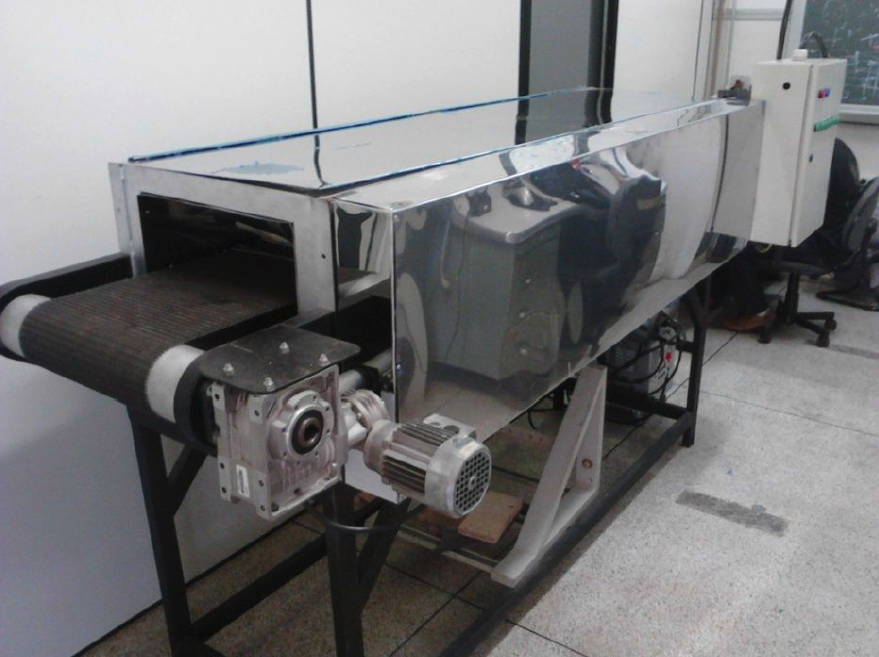
\includegraphics[width=\textwidth]{Figuras/forno_real}
\caption{Forno de esteira em escala - LAFAC}
\label{fig:forno_real}
\end{figure}

O forno possui 2,0 metros de comprimento por 0,5 metros de altura e largura, sendo revestido externamente por aço inox e placas de cerâmica refratária, como pode ser visto na figura \ref{fig:forno_frontal}. O espaço interno do forno possui  2,0 metros de comprimento por 0,4 metros de altura e largura, espaço este que possui duas áreas principais, o topo e o lastro, que estão separados pelas esteira de transporte. A esteira é circular e tanto a entrada, como a saída do forno são abertas.

\begin{figure}[H]
\centering
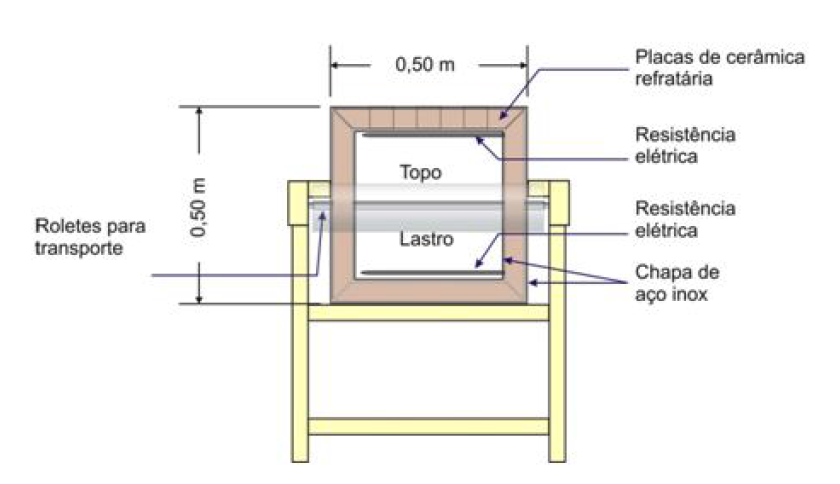
\includegraphics[width=\textwidth]{Figuras/forno_frontal}
\caption{Vista frontal forno. Adaptado de \citet{arthur}}
\label{fig:forno_frontal}
\end{figure}

O aquecimento do forno é feito por resistências que estão posicionadas ao longo da parte superior e inferior do forno de forma contínua. As ligações das resistências são separadas de forma a se controlar individualmente cada um dos 6 setores ilustrados pela figura \ref{fig:forno_esquema_lateral}, com os setores de 1 à 3 na parte superior e de 4 a 6 na parte inferior. 

\begin{figure}[H]
\centering
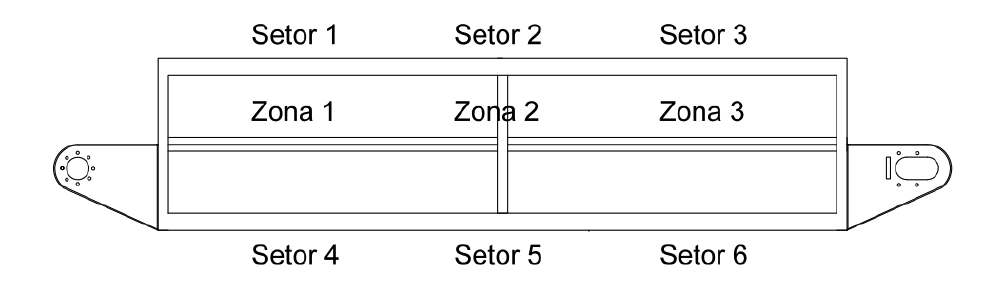
\includegraphics[width=\textwidth]{Figuras/forno_esquema_lateral}
\caption{Vista lateral do forno. Adaptado de \citet{arthur}}
\label{fig:forno_esquema_lateral}
\end{figure}

Seis sensores de temperatura termopar tipo K estão posicionados nos setores de 1 à 3 em ambos os lados do forno estão acoplados a amplificadores com compensação de junção fria AD595. Uma unidade controladora recebe os dados dos sensores por um barramento $I^2C$ e envia por radiofrequência as informações para uma estação de controle. As informações a respeito da velocidade da esteira e potência em cada uma das zonas de aquecimento também são recebidas por radiofrequência pela estação controladora.

 \section{Perfil de Temperatura no forno}
 
A unidade controladora recebe continuamente os dados da temperatura dos seis sensores localizados nas zonas 1, 2 e 3. Estes dados de temperatura, juntamente com a potência em cada uma das resistências formam as condições de contorno da simulação numérica, que calculará a temperatura em outros locais do forno. 

Para se comparar os valores calculados com a temperatura real em função da posição, um sensor termopar se deve mover dentro do forno. Como a temperatura do forno é muito acima da suportada pelos componentes eletrônicos em geral, um invólucro de cimento refratário foi utilizado para proteger o sensor e o circuito eletrônico adjacente (figura \ref{fig:envoltorio_sensor}).

\begin{figure}[H]
\centering
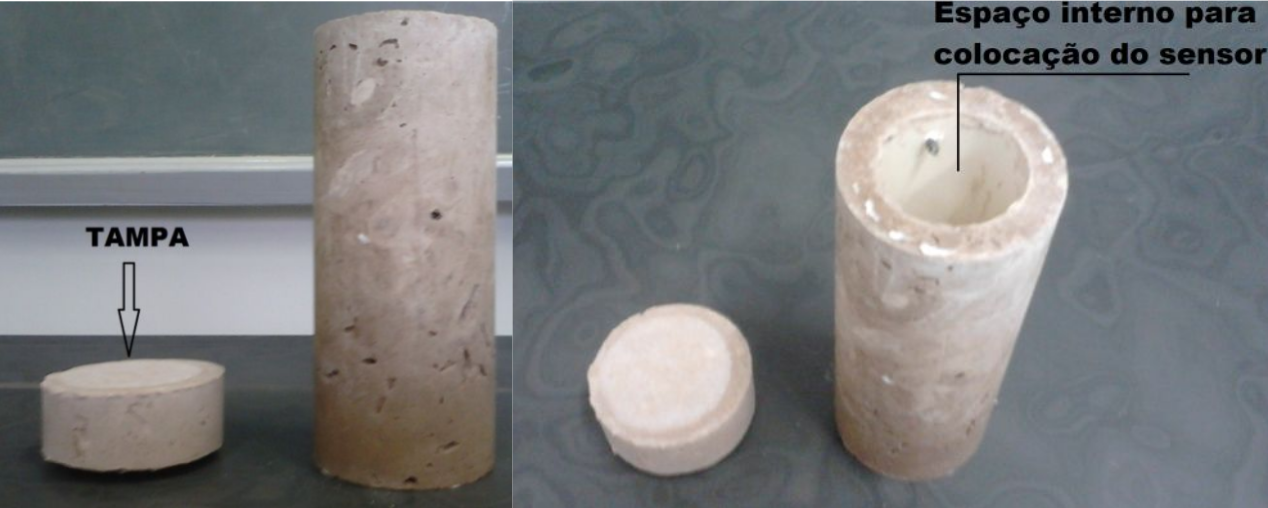
\includegraphics[width=\textwidth]{Figuras/envoltorio_sensor}
\caption{Envoltório refratário para sensor de temperatura embarcado (Figura \ref{fig:sensor_termeratura}). Adaptado de \citet{arthur}}
\label{fig:envoltorio_sensor}
\end{figure}

O circuito consiste em um termopar tipo K com um amplificador com compensação de junção fria AD595, cujos dados são recebidos por um microcontrolador PIC12F675 e enviados por um módulo transceptor de radiofrequência (figura \ref{fig:sensor_termeratura}), para que a informação possa ser coletada por um computador nas proximidades do forno.
 
\begin{figure}[H]
\centering
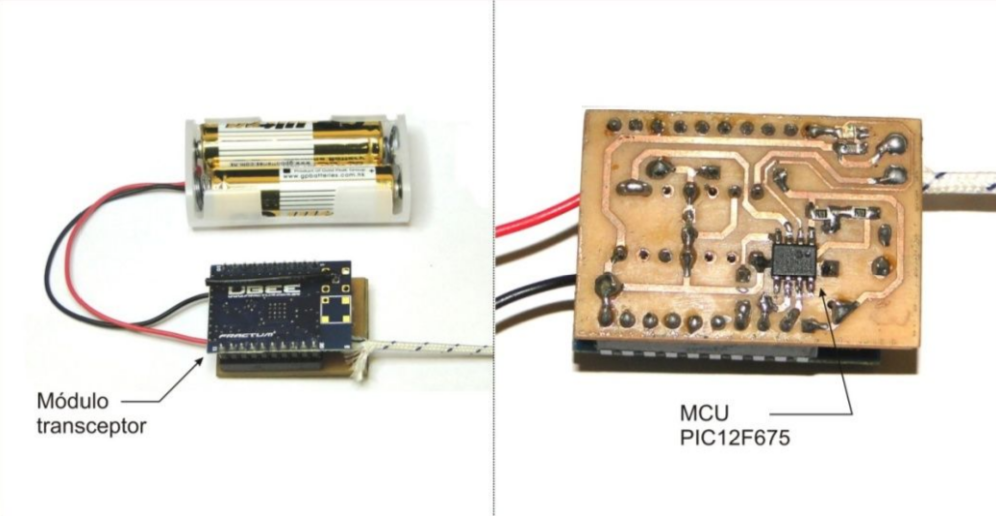
\includegraphics[width=\textwidth]{Figuras/sensor_termeratura}
\caption{Módulo transmissor com Sensor de temperatura microcontrolado. Adaptado de \citet{arthur}}
\label{fig:sensor_termeratura}
\end{figure}

O equipamento com o sensor, microcontrolador e transmissor de radio frequência mostrados pela figura \ref{fig:sensor_termeratura} foram encapsulados no envoltório de cerâmica da figura \ref{fig:envoltorio_sensor}, ficando apenas a junção do termopar no lado externo, como ilustra a figura \ref{fig:sensor_movel}.

\begin{figure}[H]
\centering
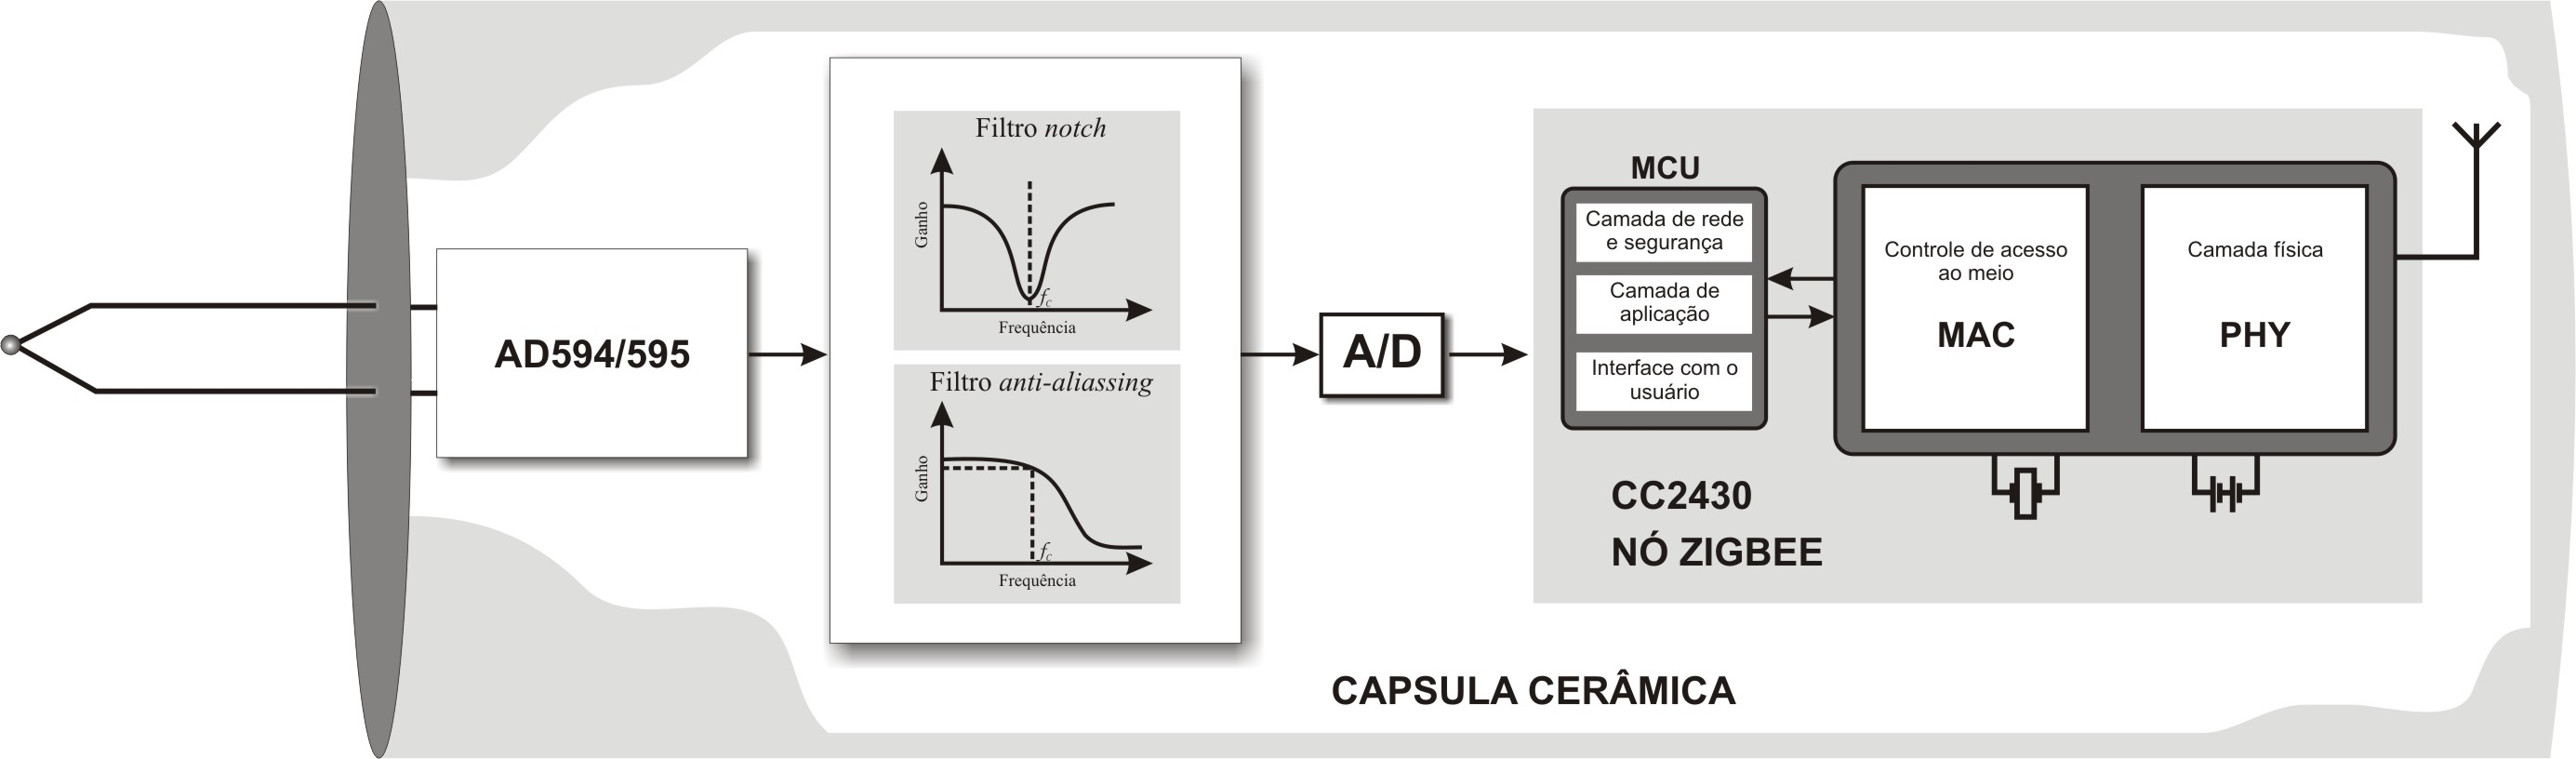
\includegraphics[width=\textwidth]{Figuras/sensor_movel}
\caption{Esquemático do sensor móvel embarcado no envoltório de cerâmica, com as funcionalidades do sensor: Amplificador e filtro, conversão analógico/digital e envio de dados por radiofrequencia}
\label{fig:sensor_movel}
\end{figure}

Alguns testes foram feitos com o sensor e o envoltório, mostrando que o processo desta metodologia, desenvolvida por \citet{arthur} funciona, dando uma noção qualitativa do comportamento da temperatura no forno em função da potencia nas zonas de aquecimento, porém mais experimentos devem ser feitos de forma sistemática para que os dados possam ser utilizados e comparados com os obtidos pela simulação. 
 
\section{Simulação da Temperatura}\label{simulação-temperatura}
 
As simulações numéricas foram feitas assumindo que a temperatura no interior do forno é dado pela equação \ref{eq:geral}, assumindo as simplificações de que não há deslocamento de ar significativo em um padrão diferente da difusão e que o estado estacionário é atingido rapidamente em comparação com as grandezas de tempo envolvidas nos processos de assamento. 

Assumindo o estado estacionário, em que $\frac{\partial T}{\partial t} = 0$, a equação a ser resolvida passa a ser a \ref{eq:simplificada} , que pode ser resolvida por diferenças finitas. Caso os resultados não sejam coerentes com os dados experimentais de temperatura dentro do forno, um novo modelo de simulação, envolvendo a circulação de ar e os efeitos da esteira será desenvolvido e testado.

\subsection{Diferenças finitas em uma Dimensão}

Para as simulações por diferenças finitas em uma dimensão, foram desconsideradas a altura e a largura do forno e levada em conta apenas a profundidade do mesmo. As equações de diferenças finitas foram resolvidas tomando como conhecida a temperatura nos três pontos dos sensores embutidos no forno e a potência irradiada pelas resistências.

O problema foi separado em duas partes, entre o sensor 1 e 2 e entre o sensor 2 e 3, de modo a utilizar como contorno externo a temperatura conhecida. As condições de contorno são portanto, de Dirichlet para a temperatura e de Neumann para o calor fornecido pelas resistências.


\subsubsection{Teste dos Algoritmos}\label{teste_alg}

Baseado nas condições de contorno descritas acima, foram desenvolvidos vários algoritmos para a resolução das equações de diferenças finitas em uma dimensão. Os algoritmos desenvolvidos estão apresentados no anexo \ref{alg:dif1d} e são baseados nos métodos de Jacobi, Gauss-Seidel, SOR e no método Direto. 

Com o intuito de se testar os algoritmos e verificar a eficiência de cada método, foi escolhida uma condição de contorno particular que apresenta uma solução analítica, a saber:

\begin{enumerate}
    \item Comprimento: 1m
    \item $T(0) = 20$
    \item $T(1) = 60$
    \item Calor inserido no sistema: $\dot{q} = 100 \cdot e^x$
\end{enumerate}

Foi testado o tempo para convergência de cada método além do número de iterações necessárias para que isto ocorresse. O teste de convergência foi feito utilizando-se como padrão a solução analítica e comparando os resultados com esta solução.


\subsubsection{Parâmetro $w$ no método SOR}

Foi desenvolvido um algoritmo utilizando o método SOR, que calcula o número de iterações para uma convergência dentro de um erro mínimo estabelecido (anexo \ref{alg:sor}). Este algoritmo repete este procedimento de convergência para uma distribuição linear de valores de $w$, mostrando o número de iterações necessárias em função do valor de $w$, para que seja encontrado o valor ótimo para $w$.

Os vales testados para $w$ foram de 1 a 2, já que 1 significaria o método de Jacobi e valores acima de 2 não dão estabilidade ao algoritmo.
 
\subsection{Eficiência computacional do algoritmo em várias linguagens}

Com o valor ótimo de $w$ encontrado, o mesmo algoritmo foi executado em várias linguagens para se descobrir qual a maneira mais rápida de se executar a simulação. 

Visto que a simulação deve ser executada em sistemas embarcados, que em sua grande maioria utilizam alguma versão de um sistema operacional Unix, foram utilizadas as linguagens C/C++, Fortran, Python e Octave para que o programa ficasse com compatibilidade cruzada, podendo ser utilizado em qualquer sistema operacional moderno. 

O programa desenvolvido para Octave pode ser executado também no Matlab e por isto o mesmo algoritmo foi testado em ambos para se comparar a performance, porém o Matlab não é Open-Source e não possui versão para a maioria dos sistemas embarcados. Os compiladores para os programas em C/C++ e Fortran foram o gcc, g++ e gfortran respectivamente.

Nas linguagens interpretadas (Octave, Matlab e Python), duas versões do algoritmo foram implementadas, uma que apresentava vetorização, utilizando os recursos nativos de operações matriciais e outra no formato das linguagens de mais baixo nível, operando ponto a ponto nos vetores.

Todos os Códigos foram executados em um AMD Xenon x4 com 8 Gb de memória RAM e um sistema operacional Linux Mint 17.


\subsection{Eficiência computacional do algoritmo em vários sistemas embarcados}

Esta será uma etapa futura do trabalho, em que será comparado o algoritmo escolhido em vários sistemas embarcados para se escolher qual o mais adequado para ser o controlador do processo.

Os sistemas embarcados que se pretende utilizar para teste são o Raspberry Pi, o BeagleBone Black, o Arduino Yun e o PCduino. Além disso, serão testadas a velocidade da simulação em microcontroladores como atmega328 e microcontroladores ARM.
 

\section{Controle}

O sistema de controle possui dois módulos que comunicam entre sim por radiofrequencia utilizando protocolo Zigbee. Para esta comunicação, foi utilizado módulos transceptores Ubee da marca fractum(R). Um dos módulos esta embutido na estação de controle da esteira, e utiliza um microcontrolador que recebe os dados dos sensores de temperatura e controla a velocidade da esteira e potência nas resistências de aquecimento (figura \ref{fig:controle_forno}). 

O outro módulo é composto por um transceptor Ubee conectado via protocolo USB ao sistema de controle que pode ser um computador um um sistema embarcado de baixo custo. Os dados da temperatura são recebidos pela unidade de controle e o algoritmo é executado para dar a resposta adequada que será enviada para o microcontrolador no Forno.
 
\begin{figure}[H]
\centering
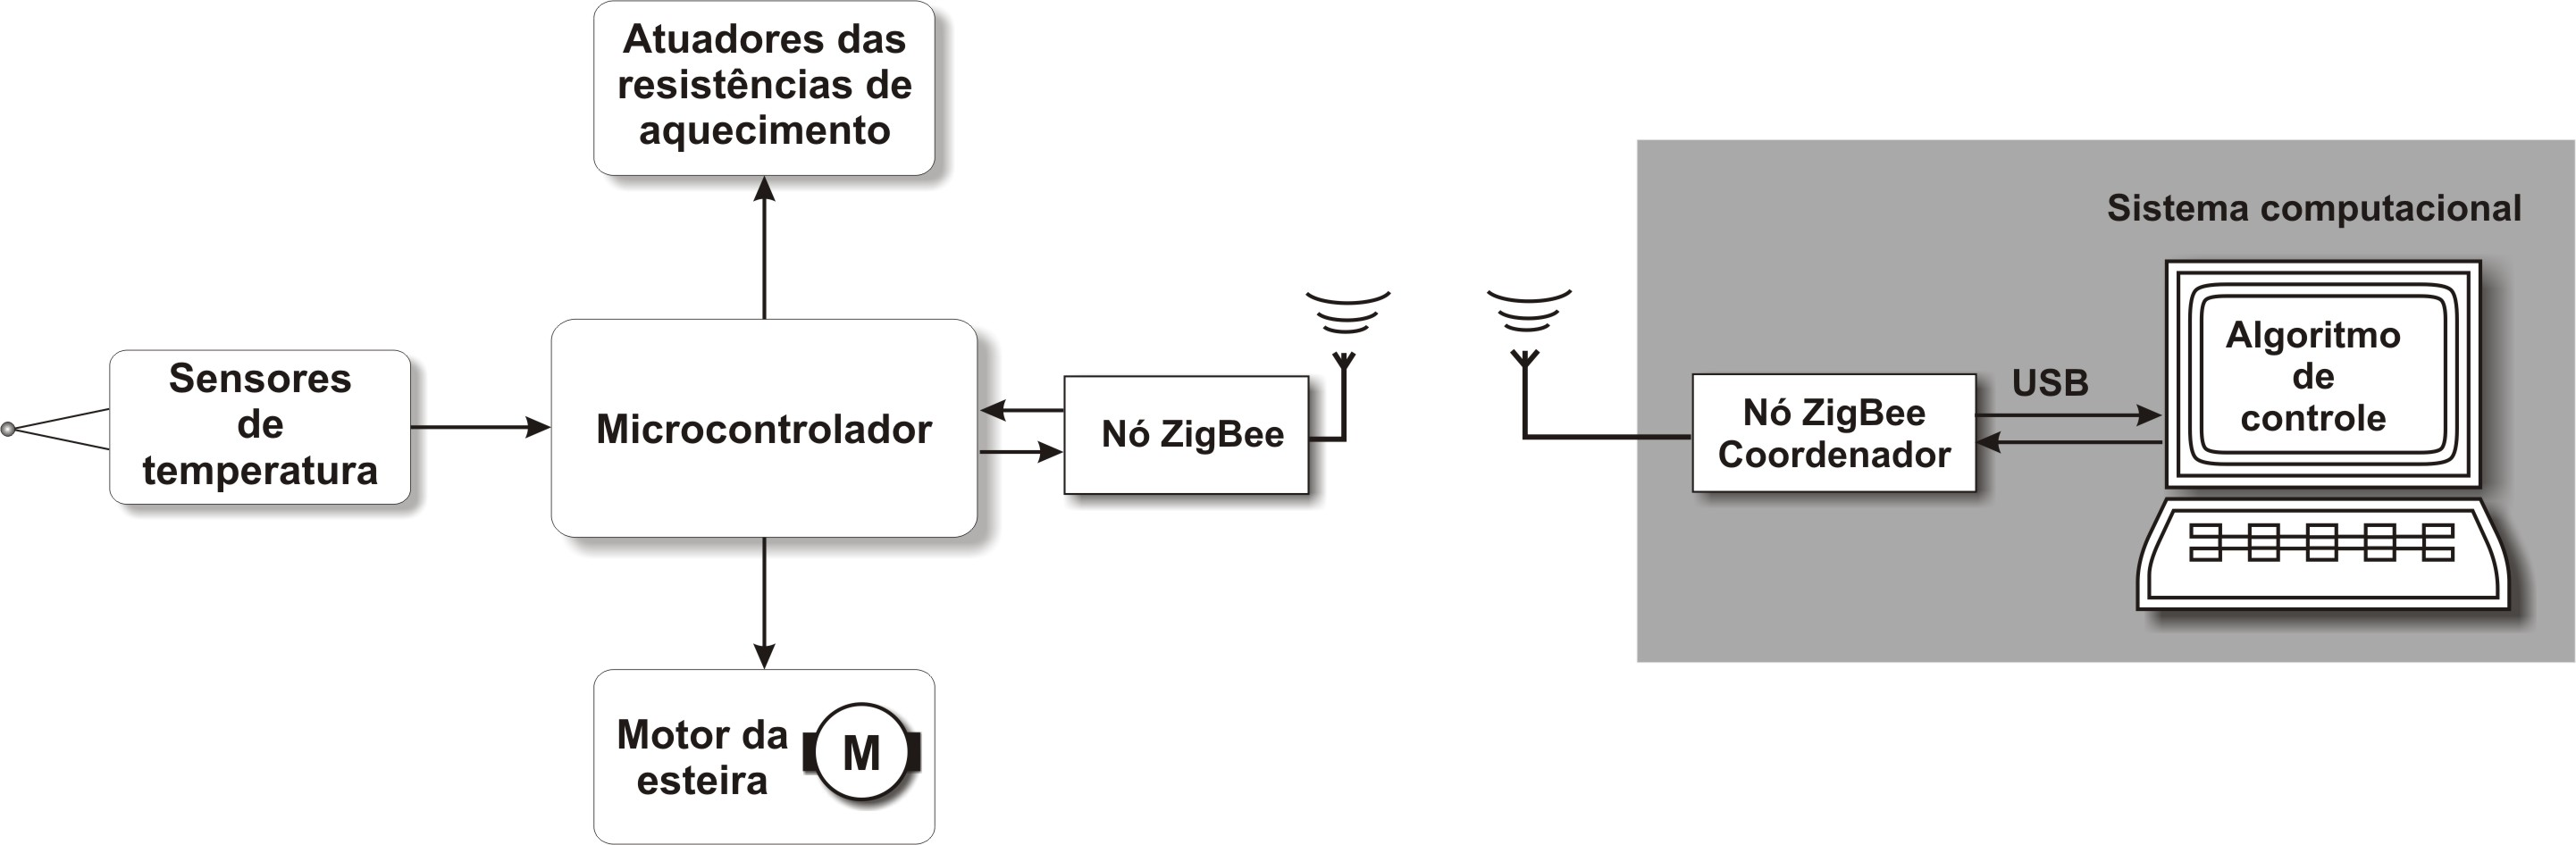
\includegraphics[width=\textwidth]{Figuras/controle_forno}
\caption{Diagrama dos módulos de controle.}
\label{fig:controle_forno}
\end{figure}
 
\subsection{Reconhecimento de Imagem}
 
Foi desenvolvido um software em Python2.7 (anexo \ref{alg:camera}, câmera), que controla uma câmera Raspicam de 5.0 MP (figura \ref{fig:raspicam}). Este software capta imagens a cada 5 segundos por intermédio de comandos na shell do sistema operacional. As imagens são então salvas e uma segunda rotina (anexo \ref{alg:camera}, reconhecimento) é chamada para analisar a mesma.

\begin{figure}[H]
\centering
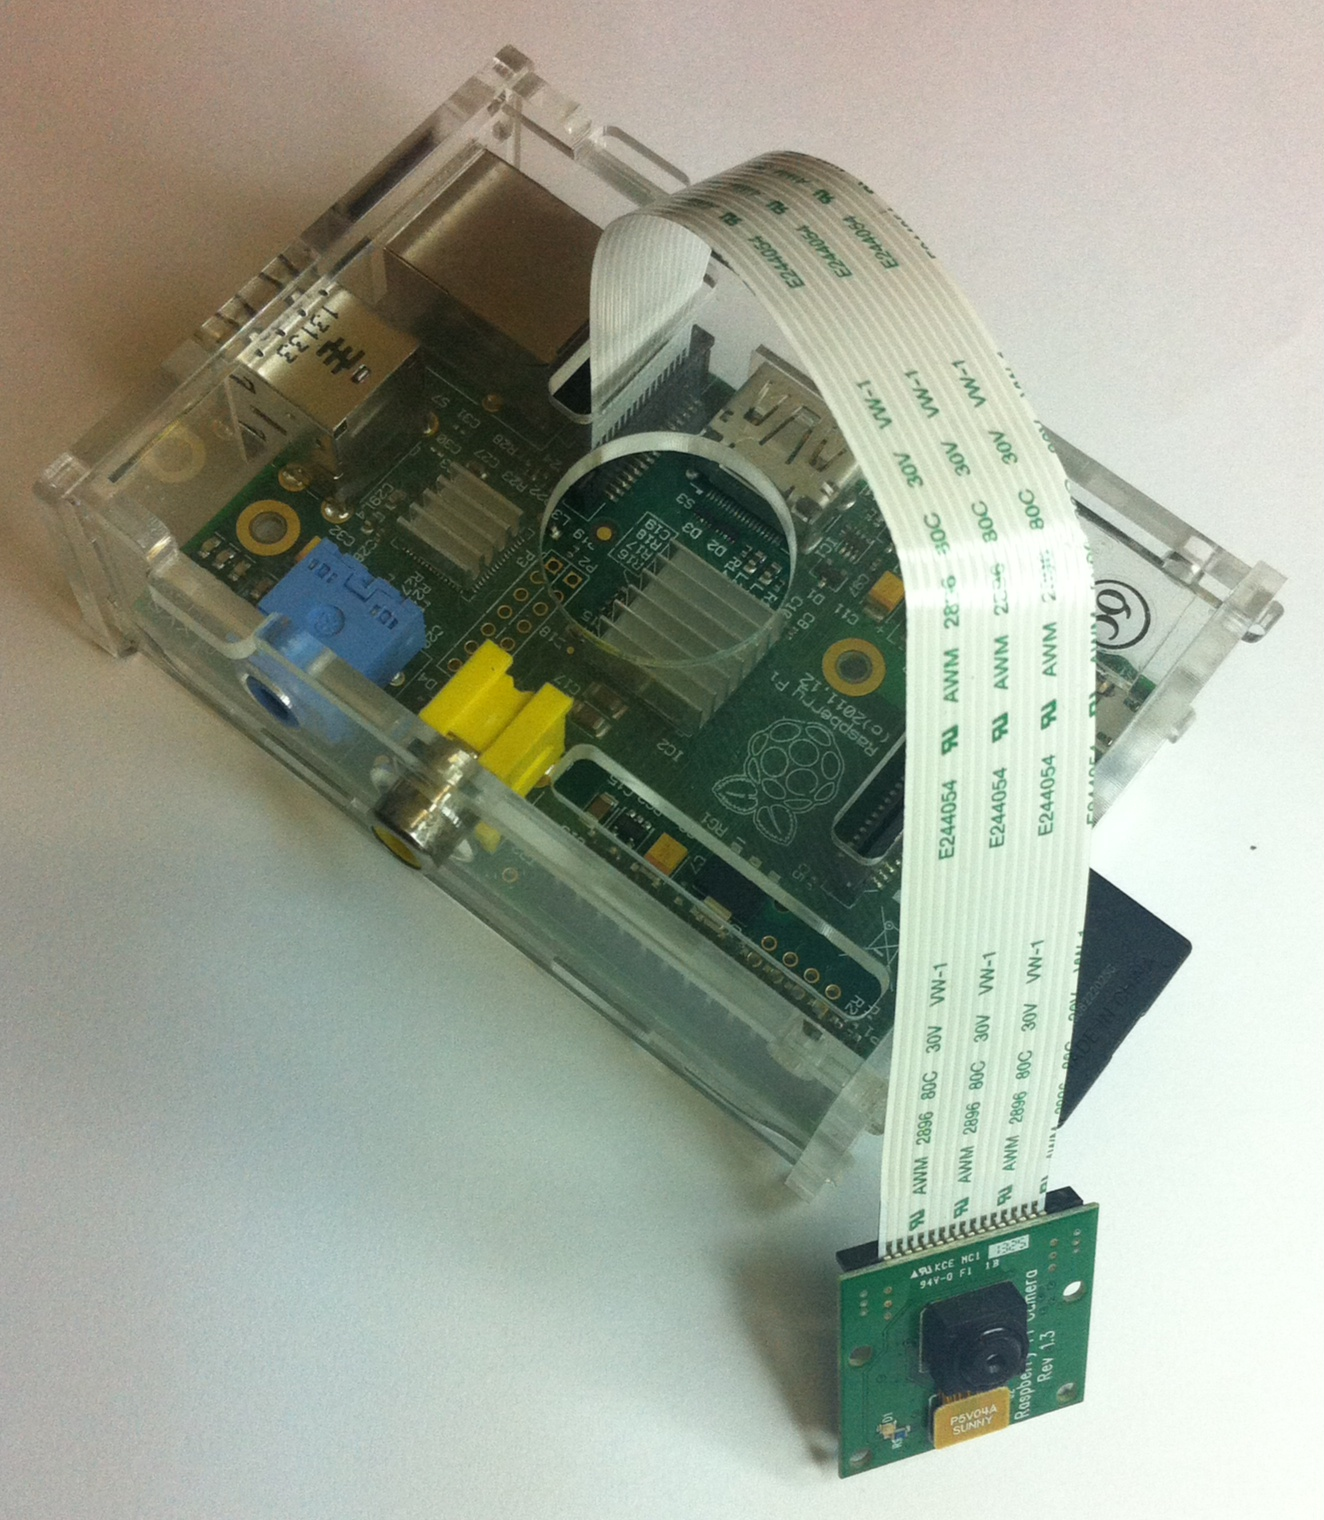
\includegraphics[width=\textwidth]{Figuras/raspicam}
\caption{Raspberry Pi com módulo câmera Raspicam 5 MP para Raspberry Pi}
\label{fig:raspicam}
\end{figure}

Este segundo script também foi desenvolvido em Python2.7 e conta com o auxílio da biblioteca de visão computacional OpenCV. Neste script, a imagem salva é tratada e analisada, retornando a quantidade de biscoitos ou bolachas que estão na entrada da esteira do forno. 

Este script possibilita que o processo de assamento seja iniciado automaticamente quando o produto chega na entrada da esteira. Outra utilidade é uma estimativa da massa total a ser assada, já que o programa retorna a área superior do alimento e a espessura é, em geral, padronizada. 

\subsection{Controle PID}

Foi escrito um algoritmo genérico de controle PID, em Python2.7, com uma classe PID que pode ser instanciada e utilizada pelo sistema de controle. 

Futuramente serão feitos experimentos para se encontrar os melhores parâmetros $K_p$, $K_i$ e $K_d$ e o controle será integrado ao sistema geral de controle

\subsection{Software de Controle - Interface Gráfica}
 
A interface gráfica foi feita utilizando a biblioteca PyQt4, que é uma extensão do Framework Qt para Python2.7. O design da interface foi feito utilizando o software QtDesigner e o resultado foi compilado utilizando o utilitário de linha de comando pyuic4.

Para que o sistema fique modular, o controle da interface foi feito em um script separado, que importa a classe da interface gráfica compilada. 

O software integra um modo manual além do modo de controle automático, permitindo que o usuário possa pausar ou alterar o processo se desejado. Pela interface, o usuário tem informação sobre a câmera na entrada do forno, quantidade de biscoitos, valor da temperatura nos sensores, a simulação térmica e também os controles manuais do forno.




